\documentclass[
	classe=$1^{ere}STI2D$,
	grayscale
]{informatique}

\usepackage{tcolorbox}

\title{Activité : les feux piétons}

\begin{document}

\maketitle
\centering{\large Manuel : situation $1$ page $160$}

\begin{tcolorbox}
	Xavier se rend au lycée à pied. Sur son chemin, il croise $4$ passages piétons.

	Chaque feu est rouge pendant $1$ minute, puis vert pendant $30$ secondes. Les feux ne sont pas synchronisés.

	Xavier n'aimant pas se lever tôt, il part au dernier moment, mais arrivera en retard si il croise $3$ feux rouges ou plus.

	\textbf{⇒ Xavier arrivera-t-il plus d'une fois sur deux en retard ?}
\end{tcolorbox}

\begin{enumerate}
	\item Lorsque Xavier rencontre un feu, quelle est la probabilité qu'il soit rouge ?
	\item On va utiliser un tableur pour simuler le trajet de Xavier. On choisit d'afficher un $1$ si le feu est rouge, et un $0$ sinon.

	      On souhaite réaliser la feuille de calcul ci-dessous :

	      \begin{center}
		      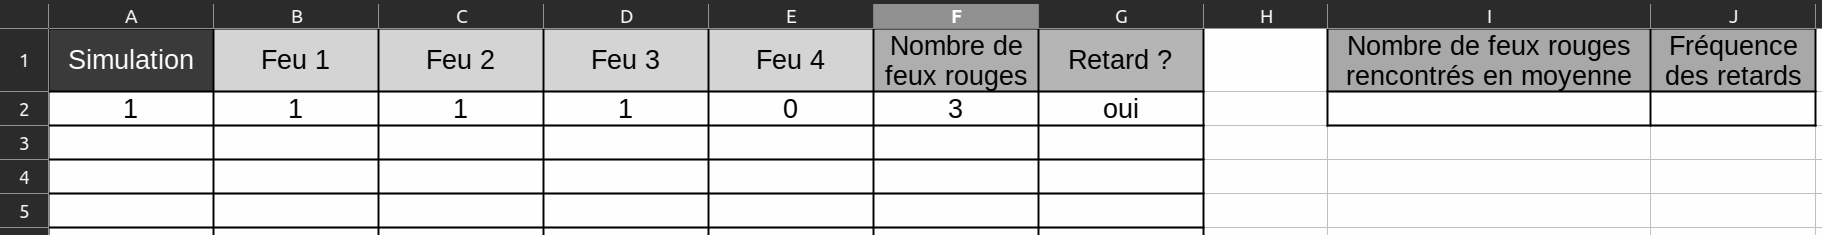
\includegraphics[width=0.9\linewidth]{Images/Tableur feux rouges (gris).png}
	      \end{center}

	      \begin{minipage}{0.5\textwidth}
		      \setlist[enumerate]{leftmargin=0em}
		      \begin{enumerate}
			      \item Dans la cellule \texttt{B2}, saisir la formule \squared{\texttt{=SI(ALEA()<=2/3 ; 1 ; 0)}}. Quel(s) résultat(s) renvoie cette fonction, et avec quelle probabilité ?

			            \correctionDots{$1$ avec proba $2/3$ $0$ avec proba $1/3$.}

			            Copier la formule dans les cellules \texttt{C2}, \texttt{D2} et \texttt{E2}.
			      \item Compléter la cellule \texttt{F2} en utilisant la fonction \texttt{SOMME}.
			      \item Compléter la cellule \texttt{G2} en utilisant la fonction \texttt{SI}.
			      \item Copier les cellules afin de réaliser $500$ simulations.
			      \item Compléter la cellule \texttt{I2}. Quel semble être le nombre moyen de feux rencontrés ? \correctionDots{$≈2,6$}
		      \end{enumerate}
	      \end{minipage}\hspace{0.02\textwidth}
	      \begin{minipage}{0.45\textwidth}
		      \begin{tcolorbox}
			      {\large\uline{AIDE TABLEUR}}


			      \setlist[itemize]{leftmargin=0.5em}
			      \begin{itemize}
				      \item \texttt{=SI(test ; "affichage 1" ; "affichage 2")} renvoie l'affichage 1 si le test est vrai, et l'affichage 2 si le test est faux.
				      \item \squared{\texttt{=SOMME(A1;A5)}} renvoie \texttt{A1 + A5}.
				      \item \squared{\texttt{=SOMME(A1:A5)}} renvoie \texttt{A1 + A2 + A3 + A4 + A5}.
				      \item La fonction \squared{\texttt{=NB.SI(A1:A12 ; 5)}} renvoie le nombre de cellules comprises entre \texttt{A1} et \texttt{A12} dont le résultat est égal à $5$.
			      \end{itemize}
		      \end{tcolorbox}
	      \end{minipage}
	\item On peut utiliser la touche \texttt{F9} pour réaliser $500$ nouvelles simulations.

	      En complétant la cellule \texttt{J2}, peut-on répondre à la question de l'énoncé ?
	\item \begin{enumerate}
		      \item \

		            \begin{minipage}{0.55\textwidth}
			            Compléter la feuille de calcul, de manière à ce que la cellule \texttt{J5} contienne le nombre de fois où $0$ feux rouges ont été rencontrés, la cellule \texttt{J6} le nombre de fois où $1$ feux rouges ont été rencontrés, etc...
		            \end{minipage}\hspace{0.02\textwidth}
		            \begin{minipage}{0.4\textwidth}
			            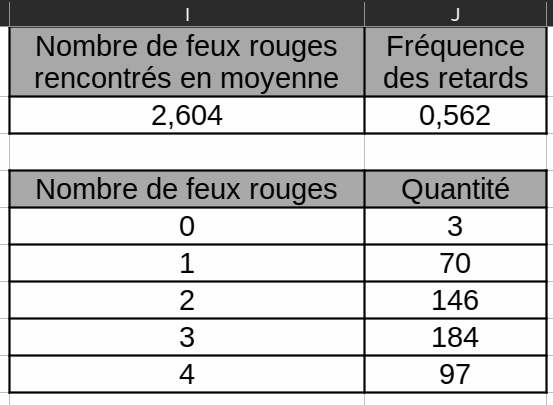
\includegraphics[width=0.9\textwidth]{Images/Tableur feux rouges + quantités (gris).png}
		            \end{minipage}
		      \item Créer un diagramme en bâtons représentant le nombre de fois où $0$, $1$, $2$, $3$ ou $4$ feux rouges ont étés rencontrés.
	      \end{enumerate}
\end{enumerate}

\end{document}